\section{Fault localization}

%% what are the claims, what are we studying, why are we studying it

\subsection{Coverage}

\rqorinsight{RQ?: Do failing tests cover different portions of the fault?}

The assumption underlying SBFL is that failing tests cover buggy portions of 
the code more than passing tests. Thus, if all failing tests cover a particular 
line of code, then that line of code is more suspicious. However, if the 
failing tests cover different portions of the buggy code, then this assumption 
no longer holds.

Therefore, for bugs that are signaled through multiple failing tests and 
require a multi-edit patch, do the different failing tests cover exactly the 
same patch locations, exactly disjoint path locations, or some combination?

Between both datasets, there are 60 total bugs that are both multi-edit and 
multi-test -- 45 in Defects4J and 15 in Bears. For each of these, we used 
Jacoco to obtain coverage for each failing test. Then we extracted the extent 
to which each test covers the patch, and we categorized the bug based on one of 
three coverage patterns: \textit{disjoint} for bugs in which no part of the 
patch is covered by all failing tests, \textit{same} for bugs in which all 
tests cover the exact same parts of the patch, and \textit{overlap} for all 
other bugs.

\todo{how do I handle line coverage vs. chunk coverage? 5 bugs is a pretty 
significant amount with these sample sizes.}

\paragraph{Results}
The overall distribution is seen in Figure \ref{fig:coverage-all}. There are 
quite 
a few more disjoint bugs \todo{how to format the words disjoint, same, and 
overlap?} than same or overlap bugs, indicating that a significant portion of 
bugs cannot be localized by only looking at parts of the program that are 
covered by all failing tests.

\begin{figure}
	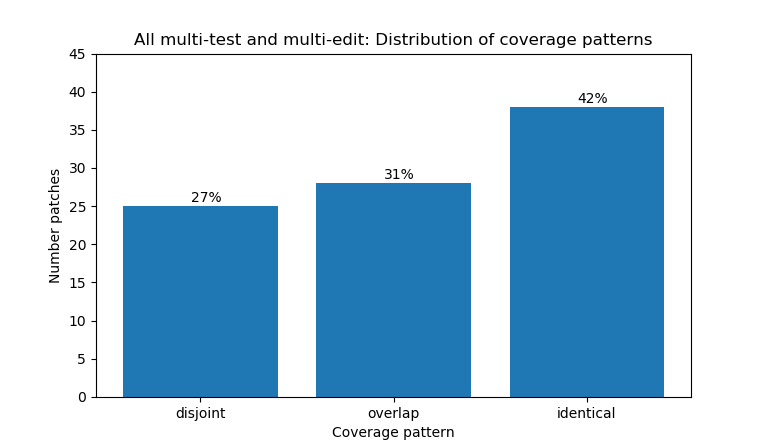
\includegraphics[width=\linewidth]{img/coverage-all.png}
	\caption{Distribution of coverage patterns for all multi-test and 
	multi-edit bugs in Bears and Defects4J}
	\label{fig:coverage-all}
\end{figure}


If we divide distribution by dataset, we can see even more interesting 
behavior. Figure \ref{fig:coverage-datasets} shows the Defects4J dataset has a 
much higher proportion of "disjoint" bugs than "overlap" bugs, while the Bears 
dataset has many more "overlap" bugs and comparatively few "disjoint" ones. We 
hypothesize that this may be due to differences in how the two datasets were 
minimized, or due to the projects used in the datasets, themselves. 
\todo{Do we have other hypotheses for why they might be different? Look at 
project level, repair types, etc.}

\begin{figure}[h]
	\label{fig:coverage-datasets}
	\begin{subfigure}{\linewidth}
		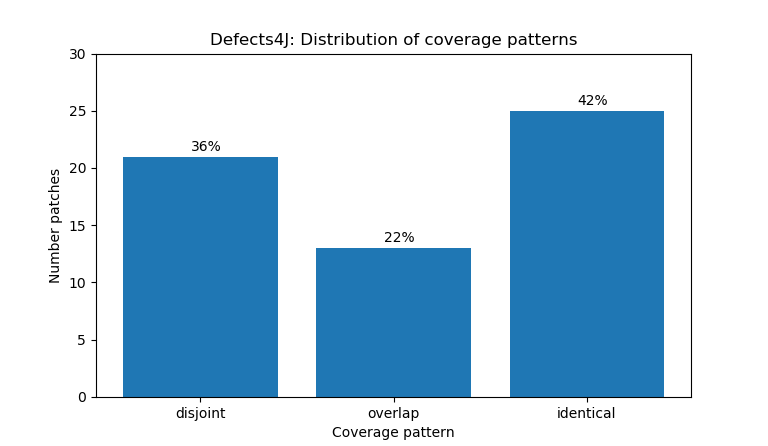
\includegraphics[width=\linewidth]{img/coverage-d4j.png}
	\end{subfigure}
	\begin{subfigure}{\linewidth}
		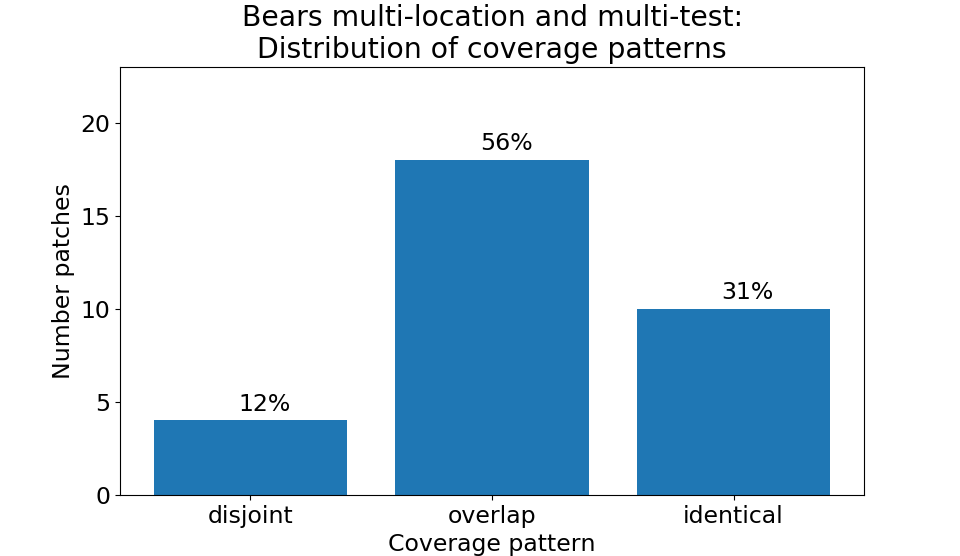
\includegraphics[width=\linewidth]{img/coverage-bears.png}
	\end{subfigure}
	\caption{Distribution of coverage patterns divided by dataset. Above is 
	Defects4J, below is Bears.}
\end{figure}

\todo{Zhen's coverage/repair tool experiment should go somewhere, maybe here}

